

\begin{frame}{Udsætning af agerhøns }

\begin{columns}[T] % T = top-aligned

\begin{column}{0.48\textwidth}
\textbf{Regler ved udsætning af agerhøns:}
\begin{itemize}
    \item Kan udsættes 1. april til 15. august
    \item Under 100 ha max 100 fugle
    \item Over 100 ha 1 fugl pr. ha
    \item Biotopplan implementeret op til 4 agerhøns pr. ha)
    \item 5-årig biotopplan 2 år inde implementeret op til max 4 agerhøns pr. ha
    \item Afvigelser fra 1 fugl pr. ha afhænger af pointsystem
    \item Alle udsætninger skal indberettes senest 1 uge efter udsætningen
\end{itemize}
\end{column}

\begin{column}{0.4\textwidth}
    % Godt billede af agerhøne eller biotop med agerhøns
    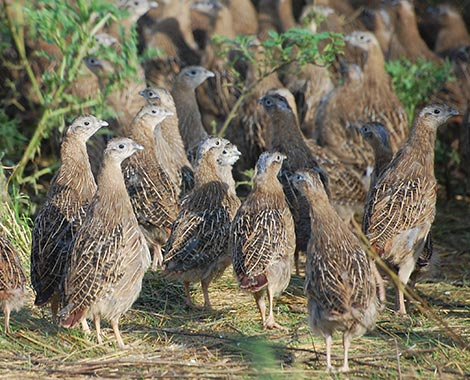
\includegraphics[width=\textwidth]{Billeder/Vildtforvaltning/udsætning/agerhøns.jpg}
    % Alternativer: agerhøne_i_mark.jpg eller vegetationsstriber_agerhoene.jpg
\end{column}

\end{columns}

\end{frame}